\documentclass{article}

\usepackage{graphicx}

\title{Apples, Bananas, and Canteloupes}
\author{Tony Li}
\date{\today}


\begin{document}
\maketitle

\begin{abstract}
	In this paper, we demonstrate a way to display scientific paper content that makes reading papers more intuitive and responsive.
\end{abstract}

\section{Introduction}
Lorem ipsum uno deux san.

\paragraph{Outline}
The remainder of this article is organized as follows:
\begin{itemize}
	\item Section~\ref{previous work} gives account of previous work.
	\item Our new and exciting results are described in Section~\ref{results}.
	\item Finally, Section~\ref{conclusions} gives the conclusions.
\end{itemize}

\section{Previous work}\label{previous work}
Once upon a time a normal paper was written: \cite{li/etal:2014}.

\section{Results}\label{results}
In this section we describe the results.  As you can see in Figure \ref{fig:plot1}, something was definitely observed.

\begin{figure}[!htbp]
	\centering
	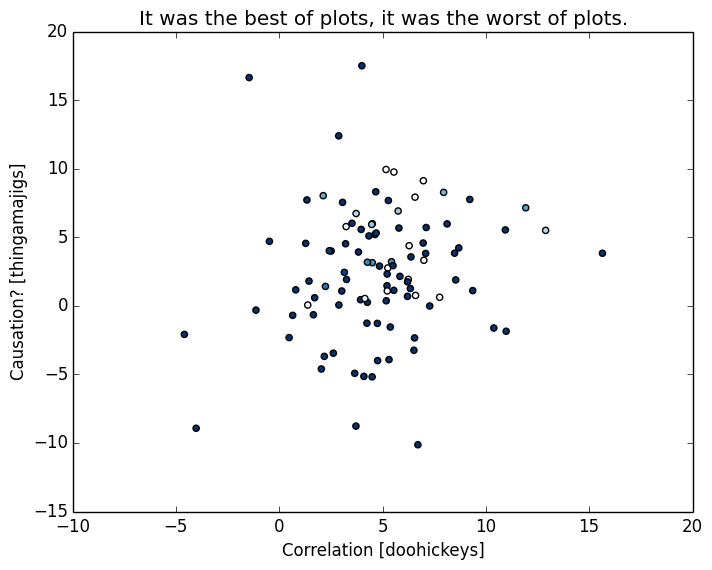
\includegraphics[width=0.8\textwidth]{plot1.png}
    \caption{Up, up, down, down, left, right, left, right, A, B, start.}
    \label{fig:plot1}
\end{figure}


\section{Conclusions}\label{conclusions}
We worked hard, and achieved very little.

\bibliographystyle{abbrv}
\bibliography{sample}

\end{document}
